\documentclass[12pt,a4paper]{book}
\usepackage[latin1]{inputenc}
\usepackage{amsmath}
\usepackage{amsfonts}
\usepackage{amssymb}
\usepackage{graphicx}
\usepackage{tikz}
\usetikzlibrary{bayesnet}
\usepackage[left=2.00cm, right=2.00cm, top=2.00cm, bottom=2.00cm]{geometry}

\begin{document}

\begin{figure}[h!]
	\centering
	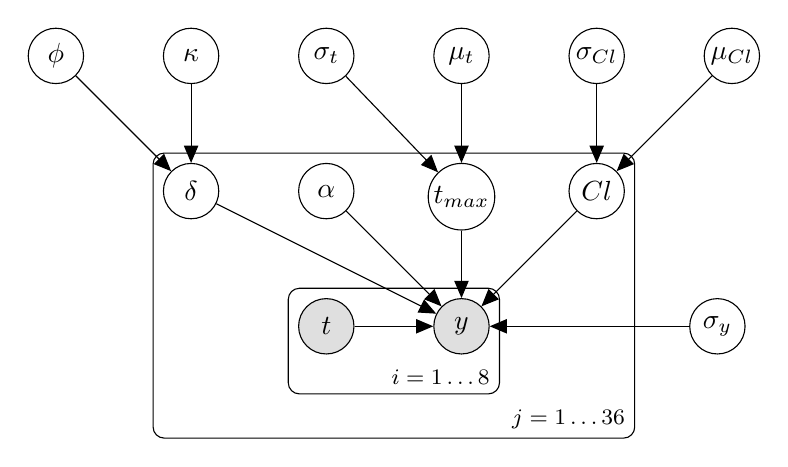
\begin{tikzpicture}
	
	\node[latent](phi){$\phi$};
	\node[latent, right=of phi](kappa){$\kappa$};
	\node[latent, right = of kappa](s_t){$\sigma_t$};
	\node[latent, right = of s_t](m_t){$\mu_t$};
	\node[latent, right = of m_t](s_cl){$\sigma_{Cl}$};
	\node[latent, right = of s_cl](m_cl){$\mu_{Cl}$};
	
	\node[latent, below = of kappa](delta){$\delta$};
	\node[latent, right = of delta](alpha){$\alpha$};
	\node[latent, below = of m_t](tmax){$t_{max}$};
	\node[latent, below = of s_cl](cl){$Cl$};
	
	\node[obs, below = of alpha](t){$t$};
	\node[obs, right = of t](y){$y$};
	\node[latent, right = of t, xshift = 3.25cm](sig){$\sigma_y$};
	
	\edge{phi}{delta};
	\edge{kappa}{delta};
	
	\edge{s_t}{tmax};
	\edge{m_t}{tmax};
	\edge{s_cl}{cl};
	\edge{m_cl}{cl};
	
	\edge{delta}{y};
	\edge{alpha}{y};
	\edge{tmax}{y};
	\edge{cl}{y};
	\edge{t}{y};
	\edge{sig}{y};
	
	\plate{t_y_pairs}{(t)(y)}{$i=1\dots 8$};
	\plate{patient_level}{(t_y_pairs)(delta)(alpha)(tmax)(cl)}{$j = 1 \dots 36$};
	\end{tikzpicture}
	\label{model_2}
\end{figure}


\end{document}